\subsection{Pagina's}\label{paginas}
In dit hoofdstuk worden een aantal pagina's beschreven zoals ontworpen in de wireframes.

\subsubsection{Pagina met inhoudsopgave}\label{paginainhoudsopgave}
Hier is geen speciaal content type voor, dit kan gedaan worden middels de aanwezige knoppen in de \emph{WYSIWYG}\seeone{wysiwyg} editor-balk. Hoe ankers aangemaakt kunnen worden staat beschreven in \emph{(Anker) links}\seeone{ankers}.

\subsubsection{Smoelenboek}\label{smoelenboek}
Het smoelenboek op het internet is een blok dat via Felix op een pagina gezet kan worden. In paragraaf \emph{Personenblok internet}\seeone{personenblokinternet} staat het te selecteren blok beschreven.

\subsubsection{Profielpagina}\label{profielpagina}

\paragraph{Gepland}

Onder deze tab op de profielpagina is de \emph{eigen} content te vinden waarvan een begin- en/of een einddatum voor is opgegeven.

\begin{center}
	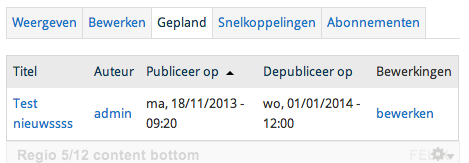
\includegraphics[scale=0.75]{img/schedulerprofile.png}
\end{center}

\paragraph{Abonnementen}

Onder deze tab is de content terug te vinden waar de gebruiker zich op geabonneerd heeft. Onder deze tab vallen drie subtabs: \emph{overzicht}, \emph{Pagina's/Reeksen} en \emph{Inhoudstypen}.

\emph{Overzicht} is het eerste scherm, in de tabel is te zien op hoeveel items de gebruiker geabonneerd is. Onder \emph{Notificatie-instellingen} kan gekozen worden of de gebruiker wel of geen notificaties wil ontvangen. Onder \emph{instellingen} kan de gebruiker instellen of hij zich automatisch wilt abonneren op nieuwe content, dat de gebruiker berichten krijgt van zijn eigen content waar hij op geaboneerd is. Met \emph{Digest mode} kan ervoor gezorgt worden dat alle meldingen in een e-mail verstuurd worden. Onder \emph{Voorkeuren} kan met de verzendingsinterval kiezen en of er een melding moet komen bij een update of bij het plaatsen van commentaar. Onder \emph{Visibility of controls} kan worden gekozen of de notificatie-instellingen al op de detailpagina te zien moeten zijn.

Onder de tab \emph{Pagina's/Reeksen} Staat een tabel met alle content waar de gebruiker op geabonneerd is en de optie om zich hiervoor af te melden.

Onder de tab \emph{Inhoudstypen} kan gekozen worden om je te abonneren op alle items van een bepaald content type.